% Generated from tex/chapters/ch04/06_構築の管理.tex for the SWEBOK structure tree
\subsubsection{ライフサイクルモデルにおける構築}

ライフサイクルモデルによって、構築の位置づけは異なる。ウォーターフォール型や段階的提供型では、要求や設計がある程度完了した後に構築が始まる。この場合、構築は主にコーディングとデバッグとして見られやすい。

一方、進化的プロトタイピングやアジャイル開発では、要求、設計、構築、テストが重なり合う。短い反復の中で、必要な要求を具体化し、設計し、コードを書き、テストする。継続的デリバリや継続的デプロイでは、コード、テスト、提供、配置がさらに密接に結びつき、自動化されたパイプラインで実行される。

\begin{figure}[htbp]
\centering
\IfFileExists{assets/generated_figures/ch04/fig-ch04-04.png}{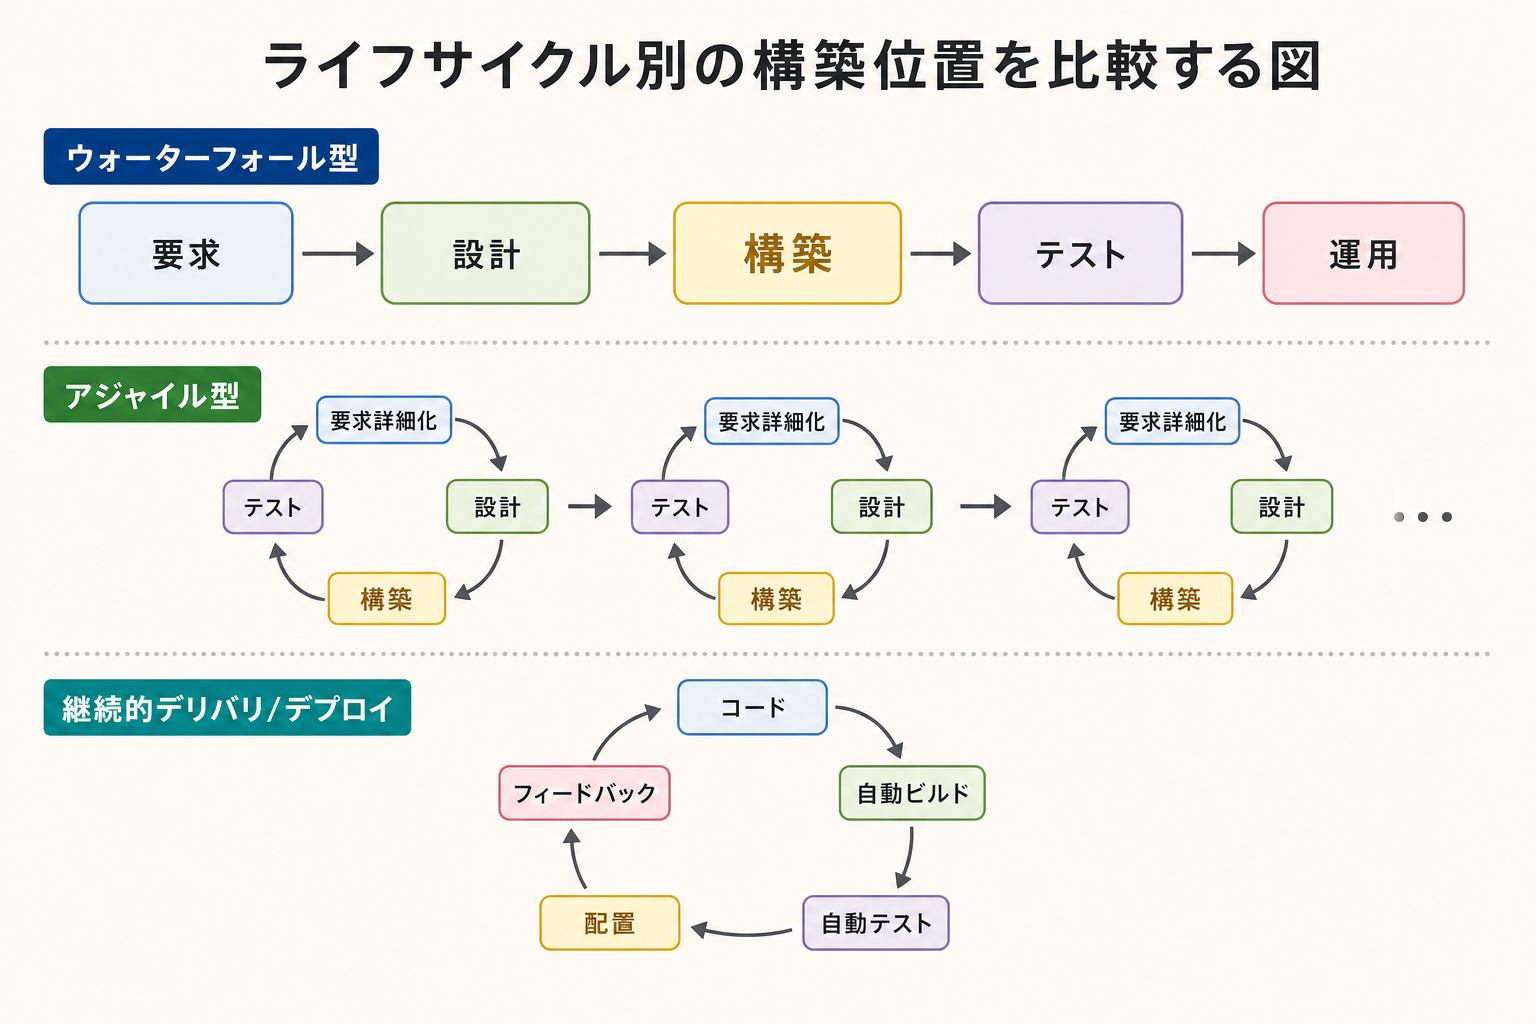
\includegraphics[width=0.96\linewidth]{assets/generated_figures/ch04/fig-ch04-04.png}}{\fbox{\parbox[c][48mm][c]{0.9\linewidth}{\centering 画像生成待ち\\ライフサイクル別の構築位置を比較する図}}}
\caption{ライフサイクル別の構築位置を比較する図}
\label{fig:ch04-04}
\end{figure}
